\documentclass[american,]{article}
\usepackage{lmodern}
\usepackage{amssymb,amsmath}
\usepackage{ifxetex,ifluatex}
\usepackage{fixltx2e} % provides \textsubscript
\ifnum 0\ifxetex 1\fi\ifluatex 1\fi=0 % if pdftex
  \usepackage[T1]{fontenc}
  \usepackage[utf8]{inputenc}
\else % if luatex or xelatex
  \ifxetex
    \usepackage{mathspec}
  \else
    \usepackage{fontspec}
  \fi
  \defaultfontfeatures{Ligatures=TeX,Scale=MatchLowercase}
\fi
% use upquote if available, for straight quotes in verbatim environments
\IfFileExists{upquote.sty}{\usepackage{upquote}}{}
% use microtype if available
\IfFileExists{microtype.sty}{%
\usepackage{microtype}
\UseMicrotypeSet[protrusion]{basicmath} % disable protrusion for tt fonts
}{}
\usepackage[margin=1in]{geometry}
\usepackage{hyperref}
\hypersetup{unicode=true,
            pdftitle={Predicting House Prices with a Linear Regression Model},
            pdfauthor={Kevin Thompson, Sterling Beason, \& Brandon Croom},
            pdfborder={0 0 0},
            breaklinks=true}
\urlstyle{same}  % don't use monospace font for urls
\ifnum 0\ifxetex 1\fi\ifluatex 1\fi=0 % if pdftex
  \usepackage[shorthands=off,main=american]{babel}
\else
  \usepackage{polyglossia}
  \setmainlanguage[variant=american]{english}
\fi
\usepackage{natbib}
\bibliographystyle{apalike}
\usepackage{longtable,booktabs}
\usepackage{graphicx,grffile}
\makeatletter
\def\maxwidth{\ifdim\Gin@nat@width>\linewidth\linewidth\else\Gin@nat@width\fi}
\def\maxheight{\ifdim\Gin@nat@height>\textheight\textheight\else\Gin@nat@height\fi}
\makeatother
% Scale images if necessary, so that they will not overflow the page
% margins by default, and it is still possible to overwrite the defaults
% using explicit options in \includegraphics[width, height, ...]{}
\setkeys{Gin}{width=\maxwidth,height=\maxheight,keepaspectratio}
\IfFileExists{parskip.sty}{%
\usepackage{parskip}
}{% else
\setlength{\parindent}{0pt}
\setlength{\parskip}{6pt plus 2pt minus 1pt}
}
\setlength{\emergencystretch}{3em}  % prevent overfull lines
\providecommand{\tightlist}{%
  \setlength{\itemsep}{0pt}\setlength{\parskip}{0pt}}
\setcounter{secnumdepth}{5}
% Redefines (sub)paragraphs to behave more like sections
\ifx\paragraph\undefined\else
\let\oldparagraph\paragraph
\renewcommand{\paragraph}[1]{\oldparagraph{#1}\mbox{}}
\fi
\ifx\subparagraph\undefined\else
\let\oldsubparagraph\subparagraph
\renewcommand{\subparagraph}[1]{\oldsubparagraph{#1}\mbox{}}
\fi

%%% Use protect on footnotes to avoid problems with footnotes in titles
\let\rmarkdownfootnote\footnote%
\def\footnote{\protect\rmarkdownfootnote}

%%% Change title format to be more compact
\usepackage{titling}

% Create subtitle command for use in maketitle
\providecommand{\subtitle}[1]{
  \posttitle{
    \begin{center}\large#1\end{center}
    }
}

\setlength{\droptitle}{-2em}

  \title{Predicting House Prices with a Linear Regression Model}
    \pretitle{\vspace{\droptitle}\centering\huge}
  \posttitle{\par}
    \author{Kevin Thompson, Sterling Beason, \& Brandon Croom}
    \preauthor{\centering\large\emph}
  \postauthor{\par}
      \predate{\centering\large\emph}
  \postdate{\par}
    \date{Data Science Program, Southern Methodist University, USA \break}

\usepackage{amsmath}
\usepackage[utf8]{inputenc}
\usepackage[T1]{fontenc}
\usepackage{setspace}
\onehalfspacing
\setcitestyle{round}
\newcommand\numberthis{\addtocounter{equation}{1}\tag{\theequation}}

\begin{document}
\maketitle
\begin{abstract}
Price prediction is pivotal for real estate. Homeowners on the sell-side
want to know when to sell, what to renovate, and how much profit they
can expect from their efforts. Homebuyers want to know whether they are
getting a fair price, where to look for homes in their budget, and the
various trade-offs that accompany a purchasing decision. Real estate
companies navigate both sides of real estate; hence, they too are a key
stakeholder. In the first part of our analysis, we estimate the
relationship between house prices, the square footage, and neighborhood
location in Ames, Iowa. In the second part of our analysis, we train a
linear regression model to predict house prices in Ames, Iowa.
\end{abstract}

\section{Introduction}\label{introduction}

Price prediction is pivotal for real estate. Homeowners on the sell-side
want to know when to sell, what to renovate, and how much profit they
can expect from their efforts. Homebuyers want to know whether they are
getting a fair price, where to look for homes in their budget, and the
various trade-offs that accompany a purchasing decision. Real estate
companies navigate both sides of real estate; hence, they too are a key
stakeholder. These stakeholders utilize multiple factors related to real
estate to determine the fair price for the property. These same factors
can be built into a model for price prediction that assists in taking
some of the guess work out of property pricing.

The analysis performed for this paper leverages a data set focused on
the housing market in Ames, Iowa. This data set is from the ``House
Prices: Advanced Regression Techniques'' Kaggle competition
(\citet{Kaggle2016}). In this competition Kaggle competitors attempt
build models that best predict housing prices based on the Ames, Iowa
data set. Over the course of this paper a similar approach to this
specific Kaggle competition will be taken. The first part of the paper
will focus on the Ames, Iowa dataset, provide the reader with detailed
information about the data and any additional variables the team created
for model building. Analysis of this data will then be performed in two
parts. In the first part of our analysis, we estimate the relationship
between house prices, the square footage, and neighborhood location in
Ames, Iowa. In the second part of our analysis, we train a linear
regression model to predict house prices in Ames, Iowa.

The intent of this paper is to provide the reader with an understanding
of how linear regression can be applied to data and the analysis that
must be undertaken to ensure a linear regression model is adequately
developed.

\citet{Sleuth}

\section{Ames, Iowa Data}\label{ames-iowa-data}

The data used for this analysis, described in the sections below, comes
from the Kaggle Competition ``House Prices: Advanced Regression
Techniques'' (\citet{Kaggle2016}). The data set for this competition
contains housing related data for Ames, Iowa. The total data set
contains 2919 observations and 80 features or variables. Although too
numerous to describe here (see the Kaggle website for full descriptors
(\citet{Kaggle2016})), these 80 features relate to quantity and quality
based attributes of a physical property that may interest any of the key
stakeholders (prospective home buyer, home seller, real estate
company/agent). For example the data provides answers to questions such
as: ``How many rooms in the property?'', ``What is the condition of the
kitchen?'', ``What is the location of the property?'', ``Is there a
basement?''. Delving deeper, the data set breaks down into 46
categorical variables and 34 numeric variables.

The categorical variables break down into a relatively equal mix of
nominal and ordinal values (23 nominal and 23 ordinal). The ordinal
variables indicate a grading of various property related components such
as the overall property quality, overall property condition, room
specific quality and room specific conditions. The nominal values
provide information on various conditions of the property such as
building materials used and dwelling type. \citet{DeCock2011}

The numeric variables contain both continuous and discrete values (20
continuous and 14 discrete). The continuous variables indicate
information a prospective stakeholder would like to understand such as
lot size, total square footage, and specific square footage for living
spaces. The discrete variables provide the prospective stakeholder with
an understanding of items such as number of bedrooms, number of
bathrooms, etc. \citet{DeCock2011}

In reviewing the data it was determined that a few variables could be
removed for reasons noted below:

\begin{itemize}
\tightlist
\item
  ID - this field is a record ID field and is not informational for
  analysis
\item
  Pool Quality - this field does not contain enough variation to be
  useful
\item
  Miscellaneous Feature - this field contains minimial information
\end{itemize}

Data quality checks were performed across all remaining variables to
address missing values, inconsistent variable names, and to ensure
consistent ordering of ordinal variables across all variables of the
same type. Comparison analysis was also performed to ensure the variable
ordering was appropriate, as shown in figures X \& X

\section{Analysis Question I}\label{analysis-question-i}

\subsection{Problem Statement}\label{problem-statement}

A local real estate company, Century 21, would like to understand the
relationship between living area of a home and sale prices.
Specifically, the company would like to focus only on sales in certain
neighborhoods (North Ames, Edwards, and Brookside). An estimate (or
estimates) of this information as well as required confidence intervals
should be provided, along with verification of the model assumptions and
addressing of suspicious observations. In the conclusion quantify the
relationship between living area and sale price with respect to these
three neighborhoods.

\subsection{Methodology and Results}\label{methodology-and-results}

We begin by fitting the following linear regression model:

\begin{equation}
Price_i = {\beta_0} + {\beta_1}GrLivArea_{i} + {\beta_2}NAmes_{i} + {\beta_3}Edwards_{i} + {\beta_4}GrLivArea_{i}\*NAmes_{i}
+ {\beta_5}GrLivArea_{i}\*Edwards_{i}
+ {\epsilon_i},
\end{equation}

where \(Price_i\) denotes the price of the i-th house, \(NAmes_i\)
denotes whether the i-th observation is located in the North Ames
neighborhood, \(GrLivArea_i\) denotes the above-ground square foot
living area for the i-th house, and \(Edwards_i\) denotes whether the
i-th observation is located in the Edwards neighborhood. The comparison
neighborhood is the Brookside neighborhood. The following two
interaction terms are included to capture the likely difference in the
marginal contribution of living area to sale price between
neighborhoods. \(\epsilon_i\) denotes the error term for the i-th
observation.

We examine a residual plot to verify the assumptions of the OLS
estimator and the hypothesis tests for the coefficients.

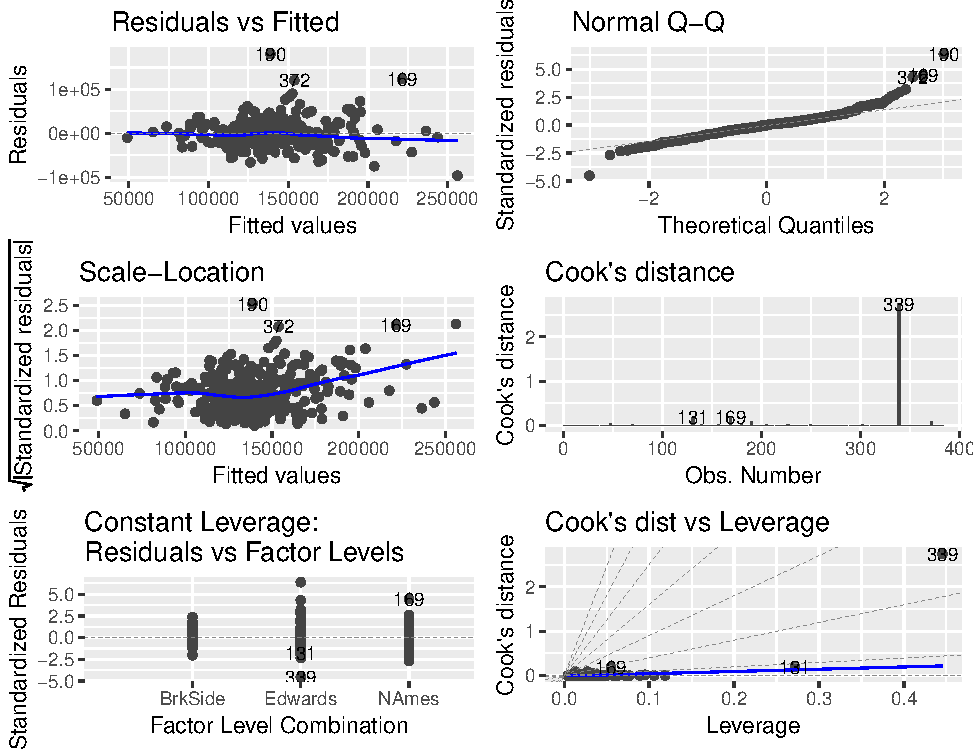
\includegraphics{HousePricesPaper_files/figure-latex/residualplot-1.pdf}

The top-right qq-plot of the studentized residuals suggests moderate
skew and the presence of influential observations. The bottom-right plot
further clarifies the influential observations of interest which have
significant leverage and distance. Regressing with and without the
observations yields significantly different results for the Edwards and
the Edwards interaction variable, which means we cannot simply ignore
it. We chose to reduce the scope of our investigation to homes with an
above ground living area of 2500 square-feet and below as the outliers
of interest have extremely large values for gross living area (98th
percentile and above). There are still outliers present after the
removal of these observations, but their removal does not impact the
results of our analysis.

We find no evidence of non-constant variance or non-linearity, while the
number of observations gives us sufficient protection from the skewness
of the residuals. We thus conclude that the linear model will suffice
for the question of interest.

\begin{verbatim}
## 
## Call:
## lm(formula = SalePrice ~ GrLivArea + Neighborhood + GrLivArea * 
##     Neighborhood, data = relevantData)
## 
## Residuals:
##    Min     1Q Median     3Q    Max 
## -96204 -14568   -310  12601 181131 
## 
## Coefficients:
##                                Estimate Std. Error t value Pr(>|t|)    
## (Intercept)                   19971.514  12351.125   1.617  0.10672    
## GrLivArea                        87.163      9.782   8.911  < 2e-16 ***
## NeighborhoodNAmes             54704.888  13882.334   3.941 9.69e-05 ***
## NeighborhoodEdwards           68381.591  13969.511   4.895 1.46e-06 ***
## GrLivArea:NeighborhoodNAmes     -32.847     10.815  -3.037  0.00256 ** 
## GrLivArea:NeighborhoodEdwards   -57.412     10.718  -5.357 1.48e-07 ***
## ---
## Signif. codes:  0 '***' 0.001 '**' 0.01 '*' 0.05 '.' 0.1 ' ' 1
## 
## Residual standard error: 28550 on 377 degrees of freedom
## Multiple R-squared:  0.4474, Adjusted R-squared:   0.44 
## F-statistic: 61.04 on 5 and 377 DF,  p-value: < 2.2e-16
\end{verbatim}

We find a positive, significant association between above-ground living
area square footage and the selling price of a home and that this
significance is maintained between neighborhoods. We estimate that a
one-hundred square foot increase in above-ground living area is
associated with a \$8716 increase in the mean selling price of a home
with a 95\% confidence interval of {[}6961, 10471{]}. We also find that
the relationship between square footage and home price changes between
neighborhoods. We estimate the change in mean price per additional 100
square-feet in North Ames to be \$3760 lower than in Brookside, while we
did not find sufficient evidence to conclude that the change in mean
price per additional 100 square-feet is different in Edwards than in
Brookside. We also similarly found that homes in North Ames are
estimated to have higher mean home values than Brookside. We estimate
the median home value in North Ames to be \$60,354 larger (95\%
confidence interval - {[}35349, 85359{]}) than Brookside, but we did not
find sufficient evidence to conclude that mean home values are different
in Edwards as opposed to Brookside. These results should not be
generalized outside of the sample, nor should we infer causal
relationships from this observational analysis.

\section{Analysis Question II}\label{analysis-question-ii}

\subsection{Problem Statement}\label{problem-statement-1}

Build a predictive model, leveraging techniques learned in DS 6371 only,
to predict sales prices of homes in all of Ames, Iowa. The goal is to
produce four models: a forward selection model, a backward selection
model, a stepwise selection model and a custom model. Each model should
have an adjusted \(R^{2}\), CV Press and Kaggle Score. In the conclusion
describe which model is best at predicting future sale prices of homes
in Ames, Iowa.

\subsection{Assumption Checks}\label{assumption-checks}

\subsection{Competing Model
Comparison}\label{competing-model-comparison}

\subsection{Parameters}\label{parameters}

\subsection{Conclusion}\label{conclusion}

\citet{Hastie2009} \citet{Trefethen1997}

\section{Appendix}\label{appendix}

\renewcommand\refname{References}
\bibliography{HousePrices.bib}


\end{document}
